

\documentclass[11pt]{article}
\usepackage[utf8]{inputenc}
\usepackage{geometry}
\usepackage{graphicx}
\usepackage{hyperref}
\usepackage{amsmath}
\usepackage{listings}
\usepackage{xcolor}
\usepackage{float}
\usepackage{subcaption}
\usepackage{algorithm}
\usepackage{algpseudocode}
\usepackage{booktabs} % For prettier tables
\usepackage{siunitx}
\usepackage{amssymb}
\usepackage{url}

% Set page margins
\geometry{a4paper, margin=1in}

% Set up code listing style
\lstset{
    basicstyle=\ttfamily,
    commentstyle=\color{gray},
    keywordstyle=\color{blue},
    stringstyle=\color{red},
    showstringspaces=false,
    captionpos=b
}

\title{Automated Lung CT Segmentation -  DICOM to UNet Analysis: Medical Imaging Coursework Report}
\author{Vishal Jain}
\date{\today}

\begin{document}

\maketitle

\tableofcontents

\newpage

\section{Introduction}
This report presents the work done for the Medical Imaging coursework. The aim of the coursework was to explore part of the LCTSC Lung CT dataset and build a 2D image segmentation model using the UNet architecture. This report will provide an overview of the steps taken, the results obtained and present a critical discussion of the results.

\section{Module 1: Handling DICOM data}
The code and the data for the analysis described in this section can be found in the \texttt{\url{src/explore_dicoms.ipynb}} notebook and the \texttt{Dataset} directory, respectively.

\subsection{Dataset Exploration}
To investigate the dicoms, the \texttt{pydicom} library was used to read the DICOM files from the different cases. The first tag that was investigated was the \texttt{PatientIdentityRemoved} tag. This tag is used to indicate whether the patient identity has been removed from the DICOM file. The tag was checked for all the cases and it was found that the value was \texttt{YES} for all cases. The next set of information that was investigated were the scanner and patient tags relevant to stratifying the data. The summary of this information is presented in Table \ref{tab:patient_meta}.

\begin{table}[h]
    \centering
    \begin{tabular}{|l|c|c|c|l|l|}
    \hline
    \textbf{Case ID} & \textbf{Sex} & \textbf{Birth Date} & \textbf{KVP} & \textbf{Model Name}          & \textbf{Manufacturer} \\ \hline
    000              & M            &                     & 120          & Sensation Open               & SIEMENS               \\ \hline
    001              & M            &                     & 120          & Sensation Open               & SIEMENS               \\ \hline
    002              & M            &                     & 120          & Sensation Open               & SIEMENS               \\ \hline
    003              & F            & 1965-06-01          & 120          & Sensation Open               & SIEMENS               \\ \hline
    004              & F            &                     & 120          & Sensation Open               & SIEMENS               \\ \hline
    005              & M            &                     & 120          & Sensation Open               & SIEMENS               \\ \hline
    006              & M            & 1977-03-03          & 120          & Sensation Open               & SIEMENS               \\ \hline
    007              & M            &                     & 120          & Sensation Open               & SIEMENS               \\ \hline
    008              & F            &                     & 120          & Sensation Open               & SIEMENS               \\ \hline
    009              & F            &                     & 120          & Biograph 40                  & SIEMENS               \\ \hline
    010              & F            &                     & 120          & Sensation Open               & SIEMENS               \\ \hline
    011              & F            &                     & 120          & Sensation Open               & SIEMENS               \\ \hline
    \end{tabular}
    \caption{Summary of patient data}
    \label{tab:patient_meta}
\end{table}

When training a model, it's crucial to ensure that both train and test sets are similarly stratified to avoid introducing bias. In this dataset, all fields except sex are consistent across cases. Although the birth date could have served as an additional stratification criterion to balance age distribution, it's only available for two patients and thus cannot be utilised. Consequently, patient sex has been used for stratification. Given the even distribution between male and female cases, no resampling techniques were required to enforce balance.

The subsequent analysis focused on voxel-related metadata. These fields were checked to ensure consistency across cases. The fields examined included voxel size, slice thickness, image orientation, rescale intercept, rescale slope, patient position, and pixel array shape. It was found that all fields were consistent across all cases except in the rescale intercept values, in which case 9 had a value of -1000 compared to the rest of the cases -1024. However, the rescale intercept is only relevant to convert the pixel values to Hounsfield units, which is not necessary for the segmentation task. The only thing that needs to be ensured is that the distribution of intensities is consistent across cases. This was checked by plotting the intensity histograms for all cases, which are shown in Figure \ref{fig:intensity_histograms}. It is important to note that the voxel intensities were winsorised to the 1st and 99th percentiles to remove outliers before plotting the histograms.

\begin{figure}[H]
    \centering
    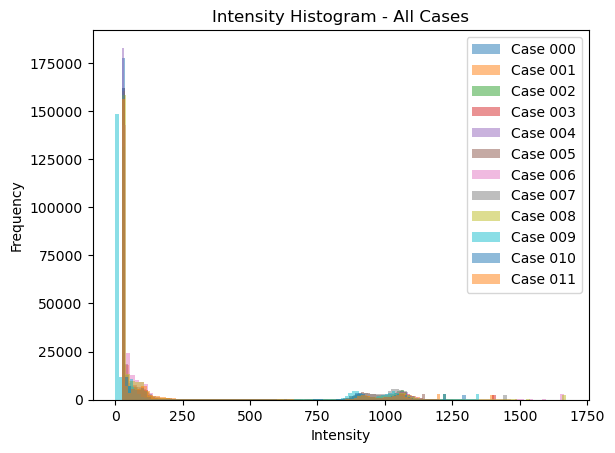
\includegraphics[width=0.8\textwidth]{figs/intensity_hist.png}
    \caption{Intensity histograms for all cases}
    \label{fig:intensity_histograms}
\end{figure}

These histograms demonstrate that the intensity distributions are consistent across the different cases in dataset. However, case 9 is identifiable by a histogram peak slightly shifted to the left relative to the peaks of other cases, illustrating a minor deviation in its intensity distribution. To correct for this, a pre processing step was introduced to winsorise and normalise the intensity distributions across all cases before training the model.

\subsection{Converting DICOMs to 3D Numpy Arrays}
The next step was to convert the DICOM files to 3D numpy arrays. The relevant code for this can be found in the \texttt{\url{src/utils.py}} script under the functions \texttt{\url{load\_npz}} and \texttt{\url{dicom\_dir\_to\_3D\_arr}}. To load the dicoms related to a single case into a 3D array the following steps were taken:
\begin{enumerate}
    \item Read all the dicom files in the directory using the \texttt{pydicom.dcmread}.
    \item Sort the files by their $z$ coordinate using the 3rd element of the \texttt{\url{ImagePositionPatient}} attribute.
    \item Extract the pixel array from each dicom file using the \texttt{pixel\_array} attribute.
    \item Use \texttt{numpy.stack} function to stack the 2d pixel arrays sorted by their $z$ coordinate along a new axis to create a 3D numpy array.
\end{enumerate} To load the masks which were provided in the form of a \texttt{.npz} file, 
\texttt{numpy.load} function was used to load the file and extract the mask array.

To verify proper alignment between the 3D image and mask arrays, they were reviewed in ITKSNAP, a standard medical image viewer. Due to ITKSNAP's format limitations, the .npz mask files could not be loaded natively and were first converted to NIfTI. Creating a NIfTI file from a numpy array necessitates specifying an affine matrix—a 4x4 matrix mapping voxel to world coordinates. Rather than deriving this matrix from DICOM metadata, both the DICOM images (which are natively viewable in ITKSNAP) and masks were converted to NIfTI using an identity affine matrix, simplifying the process. The code for which can be found in the \texttt{\url{src/utils.py}} script under the function \texttt{\url{make_niftis}}. The image and lung mask volumes were then reviewed for each case in ITKSNAP and were confirmed found to be correctly aligned by the loading process defined previosly. An example of the image and mask for case 000 is shown in Figure \ref{fig:itksnap}. It is worth noting that because the affine matrix was not derived from DICOM metadata, the images and masks were not displayed in their correct physical dimensions in ITKSNAP. However, this does not affect the segmentation process as the model is trained on the 3D numpy arrays directly, all that matters is the shape and alignment of the image and mask arrays.

\begin{figure}[H]
    \centering
    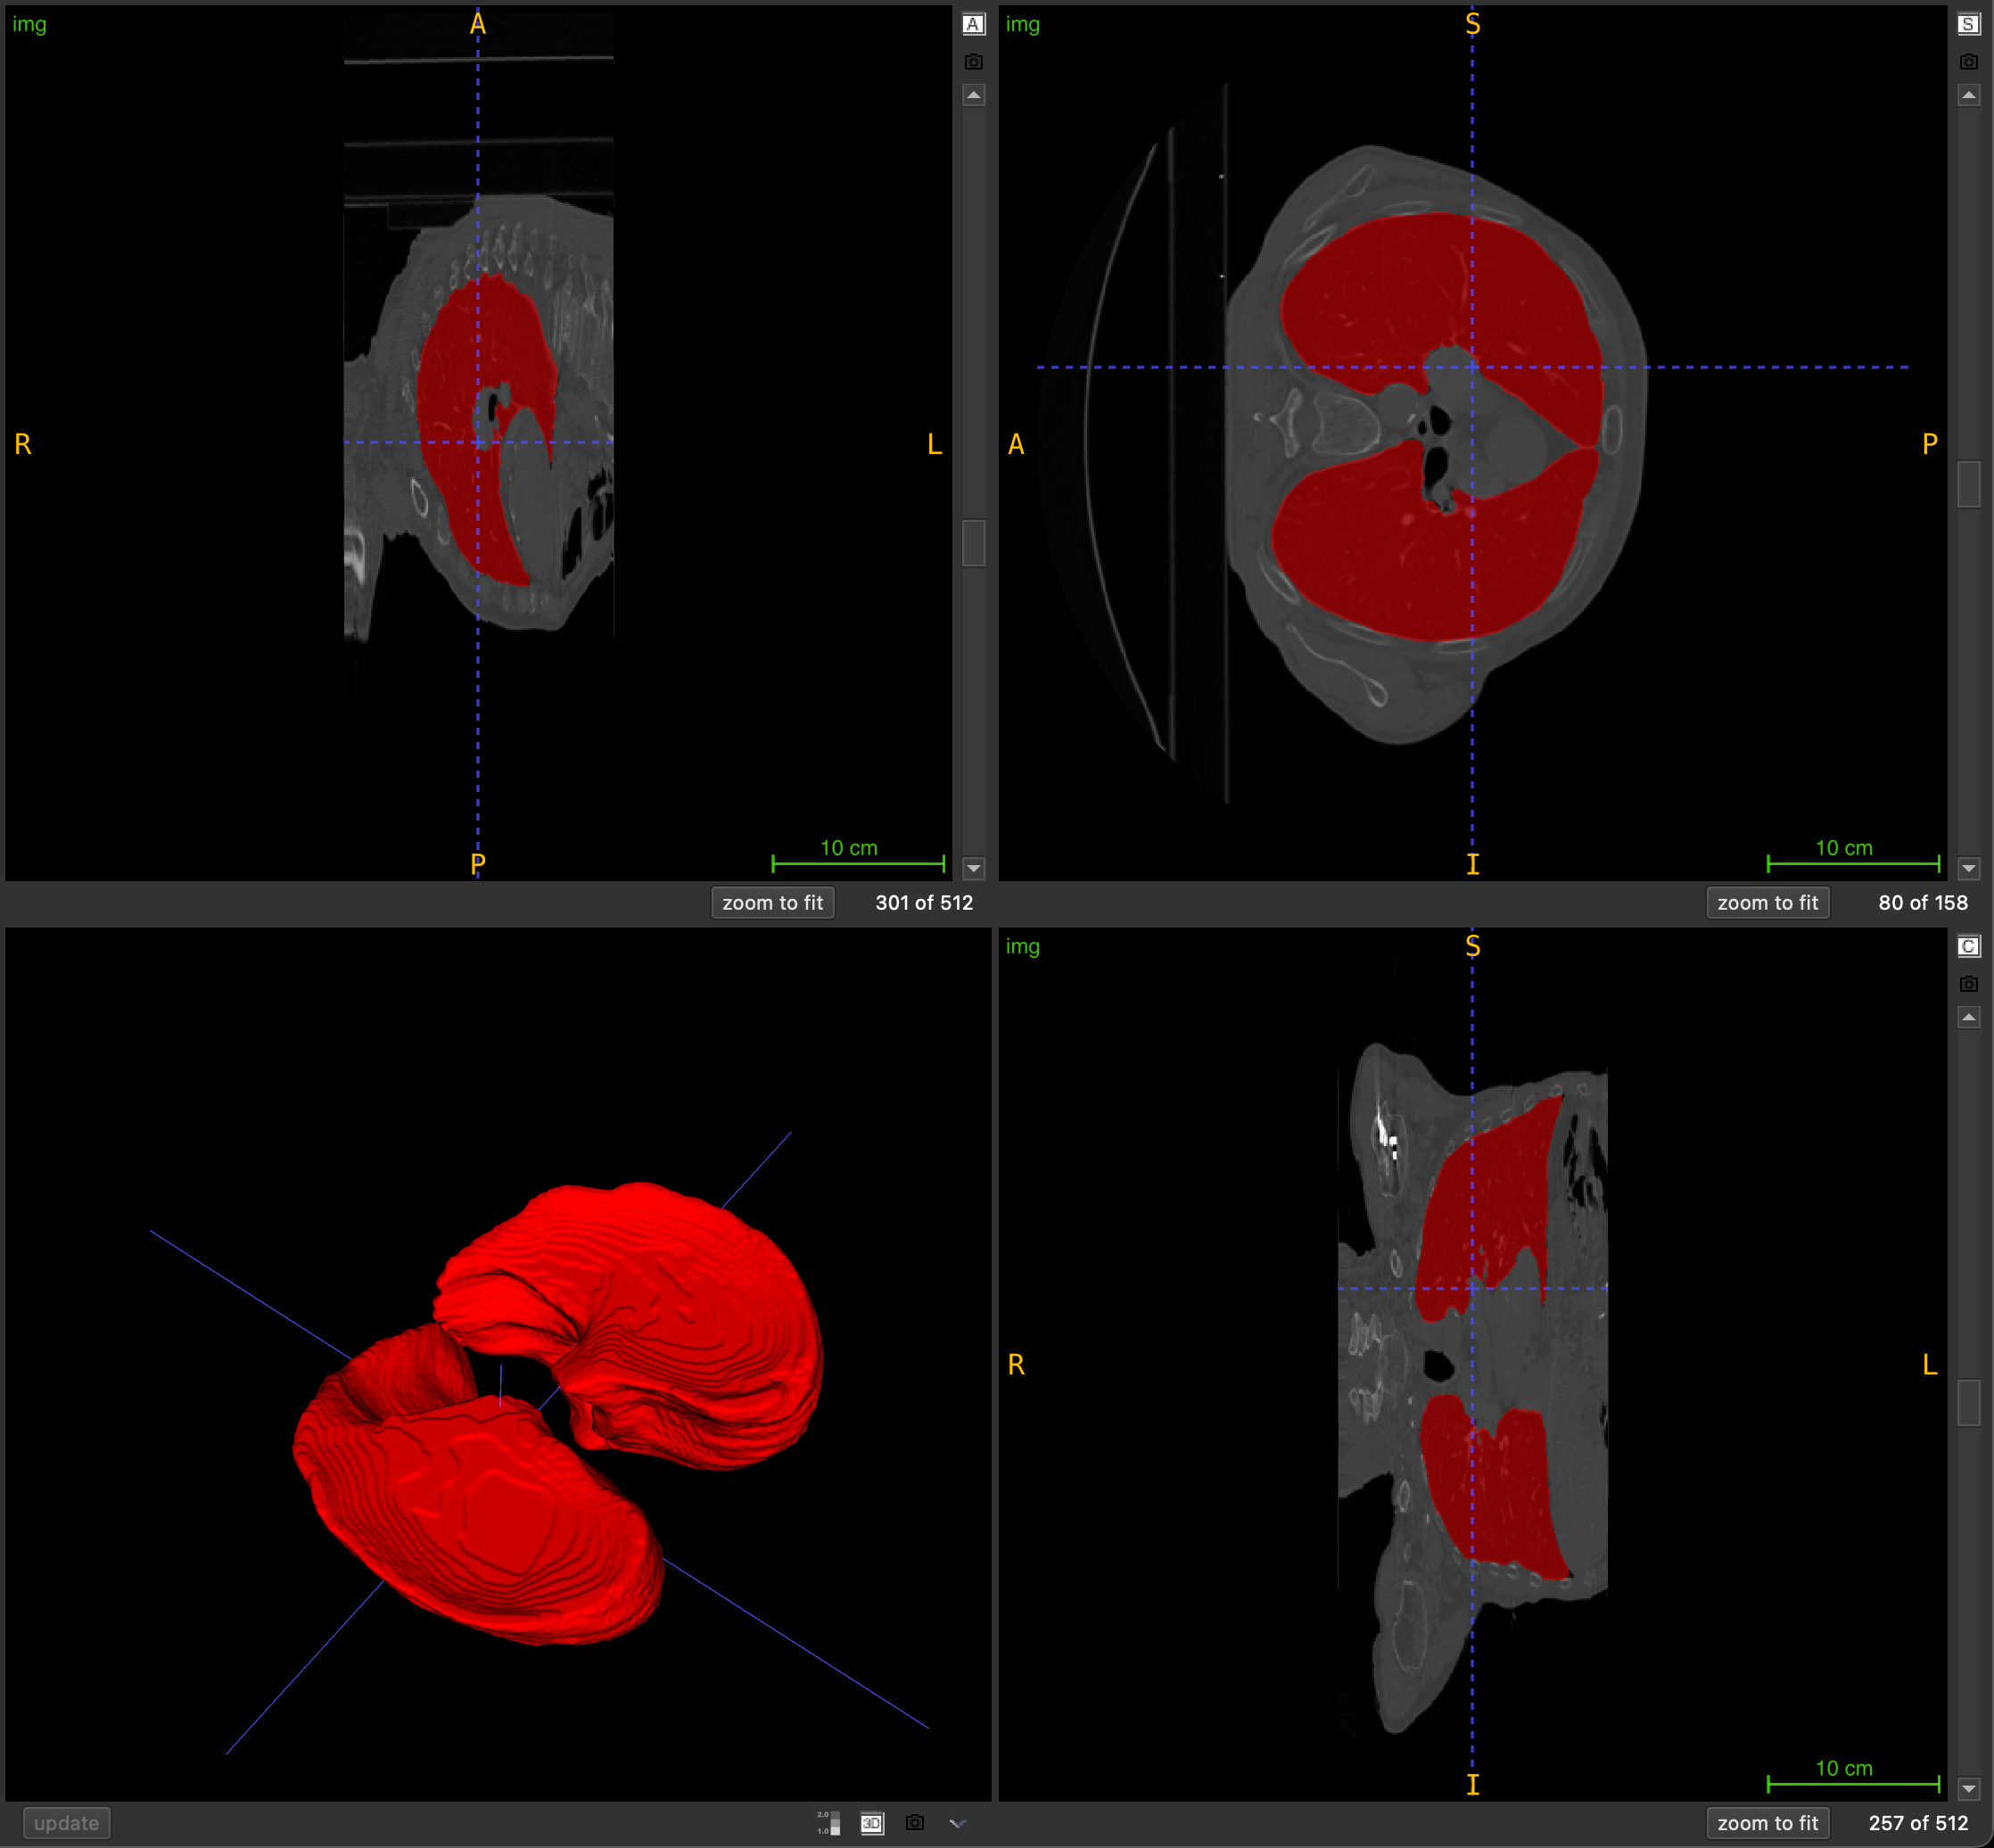
\includegraphics[width=0.8\textwidth]{figs/itksnap.png}
    \caption{ITKSNAP view of the image and mask for case 001}
    \label{fig:itksnap}
\end{figure}







\end{document}